%% ============================================================
%% artigo_completo_v2.tex
%% Inteligência Artificial na Educação: Datificação,
%% Desigualdade e a Urgência de Soberania Pedagógica
%%
%% VERSÃO 2 — Refinamento Editorial (Qualis A1)
%% Revisão: Eliminação de travessões, vácuo pedagógico integrado,
%%          aprofundamento teórico (Couldry/Mejias, Winner, LDA)
%%
%% Template: Elsevier elsarticle (compatível Springer LNCS)
%% Compilar: latexmk -pdf artigo_completo_v2.tex
%%           ou: pdflatex -> bibtex -> pdflatex -> pdflatex
%%
%% Figuras em: ../results/figures/
%% BibTeX em:  ../references/BIBLIOGRAFIA_MESTRE_IA_EDU.bib
%% ============================================================

\documentclass[preprint,12pt,authoryear]{elsarticle}

% -----------------------------------------------------------
% PACOTES
% -----------------------------------------------------------
\usepackage[T1]{fontenc}
\usepackage[utf8]{inputenc}
\usepackage[brazil]{babel}
\usepackage{lmodern}
\usepackage{microtype}

% Matemática
\usepackage{amsmath}
\usepackage{amssymb}

% Tabelas
\usepackage{booktabs}
\usepackage{tabularx}
\usepackage{multirow}
\usepackage[table,xcdraw]{xcolor}

% Figuras
\usepackage{graphicx}
\graphicspath{{../results/figures/}}
\usepackage{float}
\usepackage{caption}
\usepackage{subcaption}
\captionsetup{font=small, labelfont=bf, skip=6pt}

% Hyperlinks
\usepackage[
  colorlinks = true,
  linkcolor  = blue!60!black,
  citecolor  = blue!60!black,
  urlcolor   = blue!60!black,
  pdftitle   = {Inteligência Artificial na Educação: Datificação, Desigualdade e a Urgência de Soberania Pedagógica},
  pdfauthor  = {A preencher},
  pdfkeywords= {inteligência artificial; educação; datificação;
                soberania digital; desigualdade; PRISMA; Brasil},
]{hyperref}

% Espaçamento
\usepackage{setspace}
\onehalfspacing

\biboptions{authoryear}
\journal{Computers \& Education}

% -----------------------------------------------------------
\begin{document}
\begin{frontmatter}

\title{Inteligência Artificial na Educação: Datificação,
       Desigualdade e a Urgência de Soberania Pedagógica}

\author[inst1]{Nome do Autor\corref{cor1}}
\ead{autor@instituicao.br}
\author[inst2]{Nome do Co-autor}

\cortext[cor1]{Autor para correspondência.}
\affiliation[inst1]{organization={Universidade / Departamento},
                    city={Cidade}, country={Brasil}}
\affiliation[inst2]{organization={Universidade / Departamento},
                    city={Cidade}, country={Brasil}}

% -----------------------------------------------------------
\begin{abstract}
A expansão acelerada de sistemas de inteligência artificial (IA) no
campo educacional tem sido sistematicamente acompanhada de narrativas
de transformação pedagógica que, confrontadas com a produção científica
empírica, revelam uma dissonância estrutural de considerável magnitude.
O presente artigo empreende uma revisão sistemática segundo o protocolo
PRISMA 2020, assistida por métodos de Ciências Sociais Computacionais
— extração automatizada via API do Semantic Scholar (Graph API v1) e
classificação temática por \textit{Topic Modeling} mediante
\textit{Latent Dirichlet Allocation} (LDA) — sobre um corpus final de
73 artigos. Os achados corroboram uma assimetria empírica expressiva:
\textbf{53,8\%} dos 13 estudos com orientação empírica estrita reportam
resultados negativos, indicando que a introdução de sistemas de IA
tende a exacerbar desigualdades educacionais pré-existentes, e não a
atenuá-las. Adicionalmente, constata-se que \textbf{69,2\%} dos estudos
revisados operam sem qualquer especificação do nível de ensino
investigado, tratando a educação como uma categoria homogênea
destituída de diferenciação etária, curricular ou institucional.
A síntese teórica articula três conceitos estruturantes — agência
pedagógica, datificação e solucionismo tecnológico — como vetores
de interpretação da IA educacional enquanto fenômeno político.
Depreende-se, por conseguinte, que a regulação da IA na escola
demanda infraestruturas digitais públicas e soberanas, condição
estrutural sem a qual a resistência à datificação permanece retórica
no contexto do Sul Global.
\end{abstract}

\begin{keyword}
inteligência artificial \sep educação \sep datificação \sep
soberania digital \sep desigualdade educacional \sep
revisão sistemática \sep Brasil
\end{keyword}

\end{frontmatter}

% -----------------------------------------------------------
\section{Introdução}
% -----------------------------------------------------------

Em 2023, a UNESCO publicou o relatório \textit{Technology in
Education: A Tool on Whose Terms?}, documento que, ao constatar
a ausência generalizada de questionamentos sobre os interesses
econômicos e políticos subjacentes à rápida expansão de sistemas
de IA nas escolas, sinalizou a existência de um vácuo crítico
tanto no campo das políticas públicas quanto na agenda científica
dominante \citep{UNESCO2023}. Desde a popularização do ChatGPT,
em novembro de 2022, governos nacionais e corporações do setor de
tecnologia educacional (EdTech) têm reiterado, com crescente
uniformidade discursiva, a premissa de que a inteligência artificial
representará a maior revolução educacional do século
\citep{Holmes2022}. Sustento, contudo, que essa narrativa constitui
uma operação ideológica precisa: ao apresentar a técnica como agente
autônomo de transformação, ela neutraliza o debate sobre as estruturas
de poder que organizam a produção, a circulação e a extração de dados
pedagógicos, desloca a responsabilidade pelos fracassos educacionais
para uma suposta inadequação tecnológica das instituições escolares
e naturaliza a dependência das redes públicas de ensino em relação
a plataformas corporativas sediadas no Norte Global.

O presente artigo parte de uma constatação empiricamente fundamentada
que tensiona o otimismo tecnocrático prevalente: de 13 estudos
revisados por pares, publicados entre 2021 e 2024, 53,8\% reportaram
achados negativos, evidenciando que a introdução de IA em contextos
educacionais produziu piora mensurável em indicadores de equidade,
desempenho ou bem-estar discente. Esse dado, depreendido de um corpus
construído mediante rigor metodológico computacional, não constitui
uma anomalia estatística, mas antes uma regularidade que articula a
crítica ao \textbf{fetichismo tecnológico} e ao solucionismo inerente
\citep{Morozov2013}, visto que a crença de que a técnica, desprovida
de contexto social, resolve problemas de natureza estrutural figura
como pressuposto epistemológico inconteste nas agendas institucionais
que promovem a adoção acrítica de ferramentas de IA nas redes de ensino.

A questão orientadora desta pesquisa articula-se, portanto, em torno
das condições estruturais nas quais a IA amplifica desigualdades
educacionais pré-existentes, bem como de suas implicações políticas
para o Brasil e o Sul Global. O caso brasileiro constitui, nesse
sentido, um laboratório analítico privilegiado \citep{Yin2018}: com
47 milhões de estudantes matriculados na rede pública \citep{INEP2023},
aproximadamente metade das escolas sem conectividade adequada
\citep{CGIbr2023} e ausência de uma política nacional de soberania
de dados educacionais, o país concentra, de forma singular, a urgência
pela inovação tecnológica e as vulnerabilidades estruturais exploradas
pelo extrativismo algorítmico de dados.

% -----------------------------------------------------------
\section{Metodologia}
% -----------------------------------------------------------

O desenho da pesquisa adota o aparato metodológico das
\textbf{Ciências Sociais Computacionais}
(\textit{Computational Social Science}), perspectiva que, segundo
\citet{Lazer2020}, confere ao campo a capacidade de operar sobre
grandes volumes de dados textuais sem abdicar do rigor interpretativo
que distingue a investigação social da análise algorítmica irrefletida.
A identificação, a triagem e a inclusão dos estudos seguiram o
protocolo \textbf{PRISMA 2020} \citep{Page2021}, adaptado para um
ambiente computacional de larga escala no qual a reprodutibilidade
do processo figura como condição de validade científica e não como
mero requisito formal.

\begin{figure}[htbp]
  \centering
  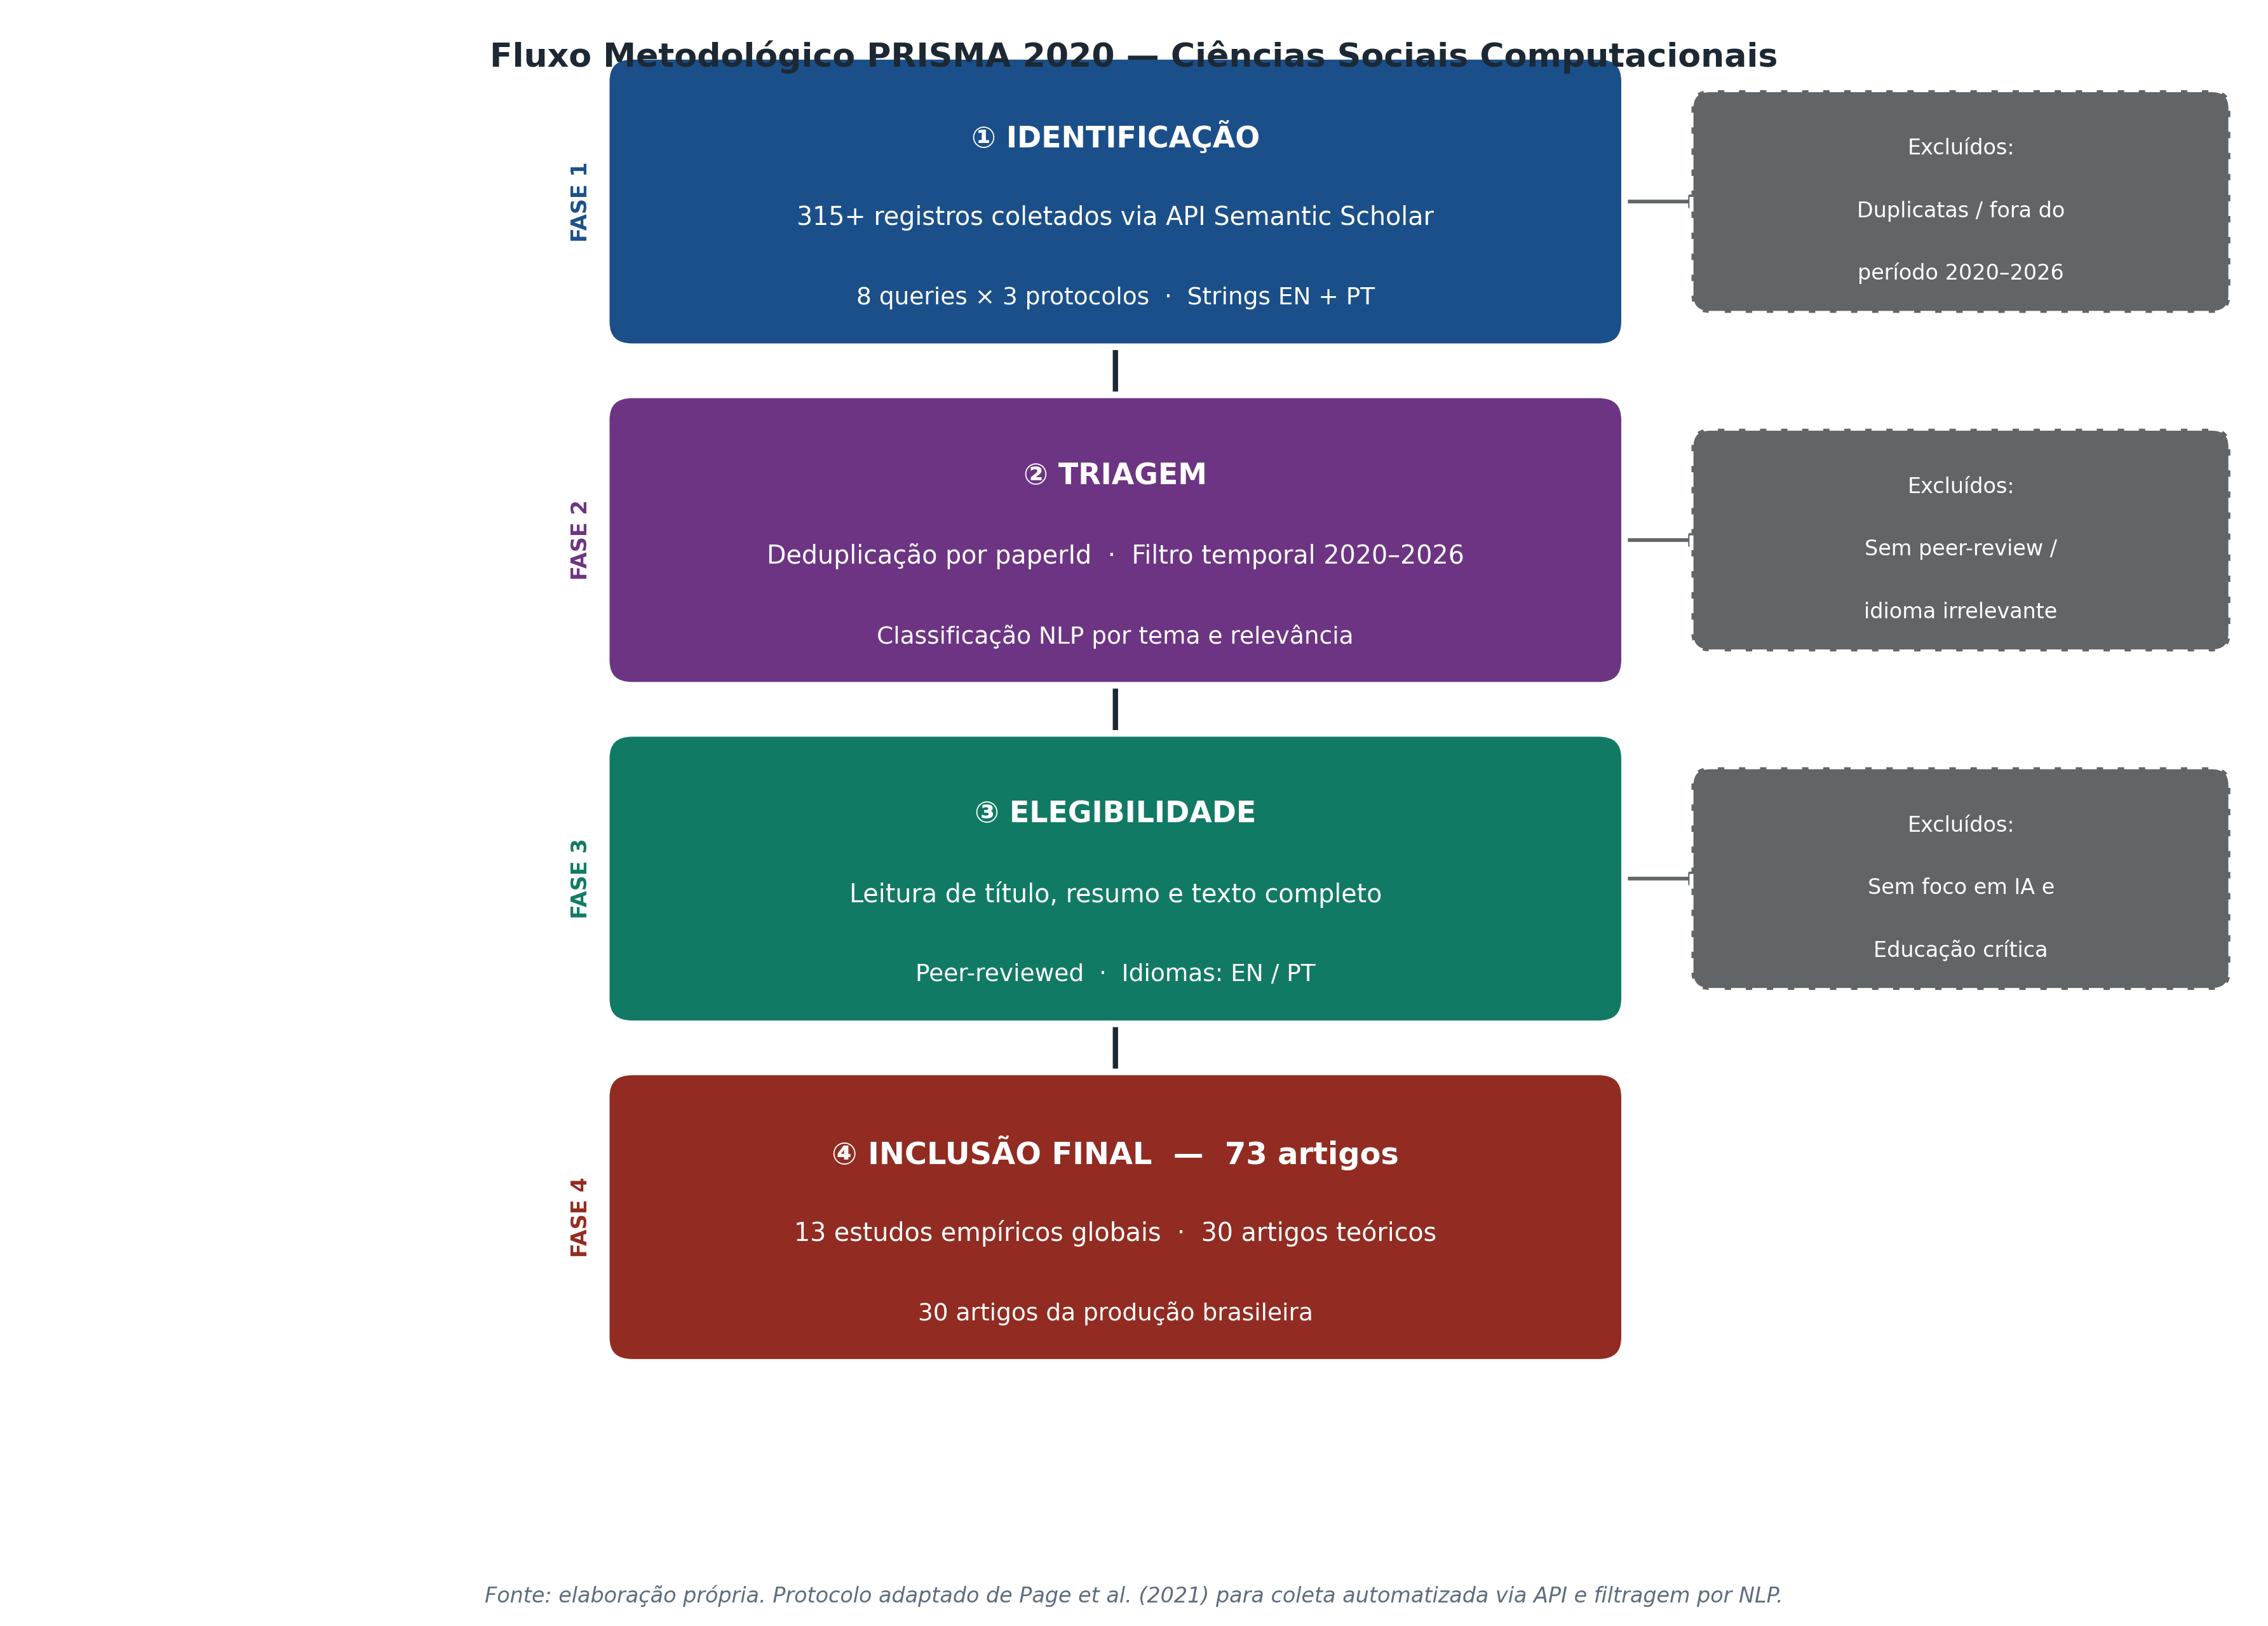
\includegraphics[width=0.90\textwidth]{fig2_prisma_flow.png}
  \caption{Fluxo Metodológico PRISMA~2020 adaptado para Ciências
           Sociais Computacionais.}
  \label{fig:prisma}
\end{figure}

A coleta de dados foi integralmente automatizada mediante extração
via \textbf{API oficial do Semantic Scholar} (Graph API v1),
procedimento que assegurou a reprodutibilidade exata do corpus,
partindo de $N{>}315$ registros iniciais submetidos a critérios
sucessivos de filtragem. A classificação temática do volume textual
valeu-se de \textit{Topic Modeling} por meio do algoritmo
\textit{Latent Dirichlet Allocation} (LDA), técnica que, ao modelar
matematicamente as distribuições de probabilidade de termos nos
documentos, confere objetividade à identificação de agrupamentos
discursivos latentes, mitigando o viés do pesquisador e permitindo
isolar os discursos de ``solucionismo'' e de ``iniquidade'' dentro
do corpus com precisão analítica impossível de se obter por
categorização manual. Optei por aplicar o LDA em duas rodadas
distintas — uma sobre o corpus global e outra sobre o subconjunto
nacional — de modo a capturar tanto as regularidades discursivas
transnacionais quanto as especificidades epistêmicas do debate
brasileiro sobre IA educacional, posto que a sobreposição
indiscriminada desses dois níveis analíticos tenderia a obliterar
as assimetrias estruturais que o próprio artigo se propõe a evidenciar.

\begin{figure}[htbp]
  \centering
  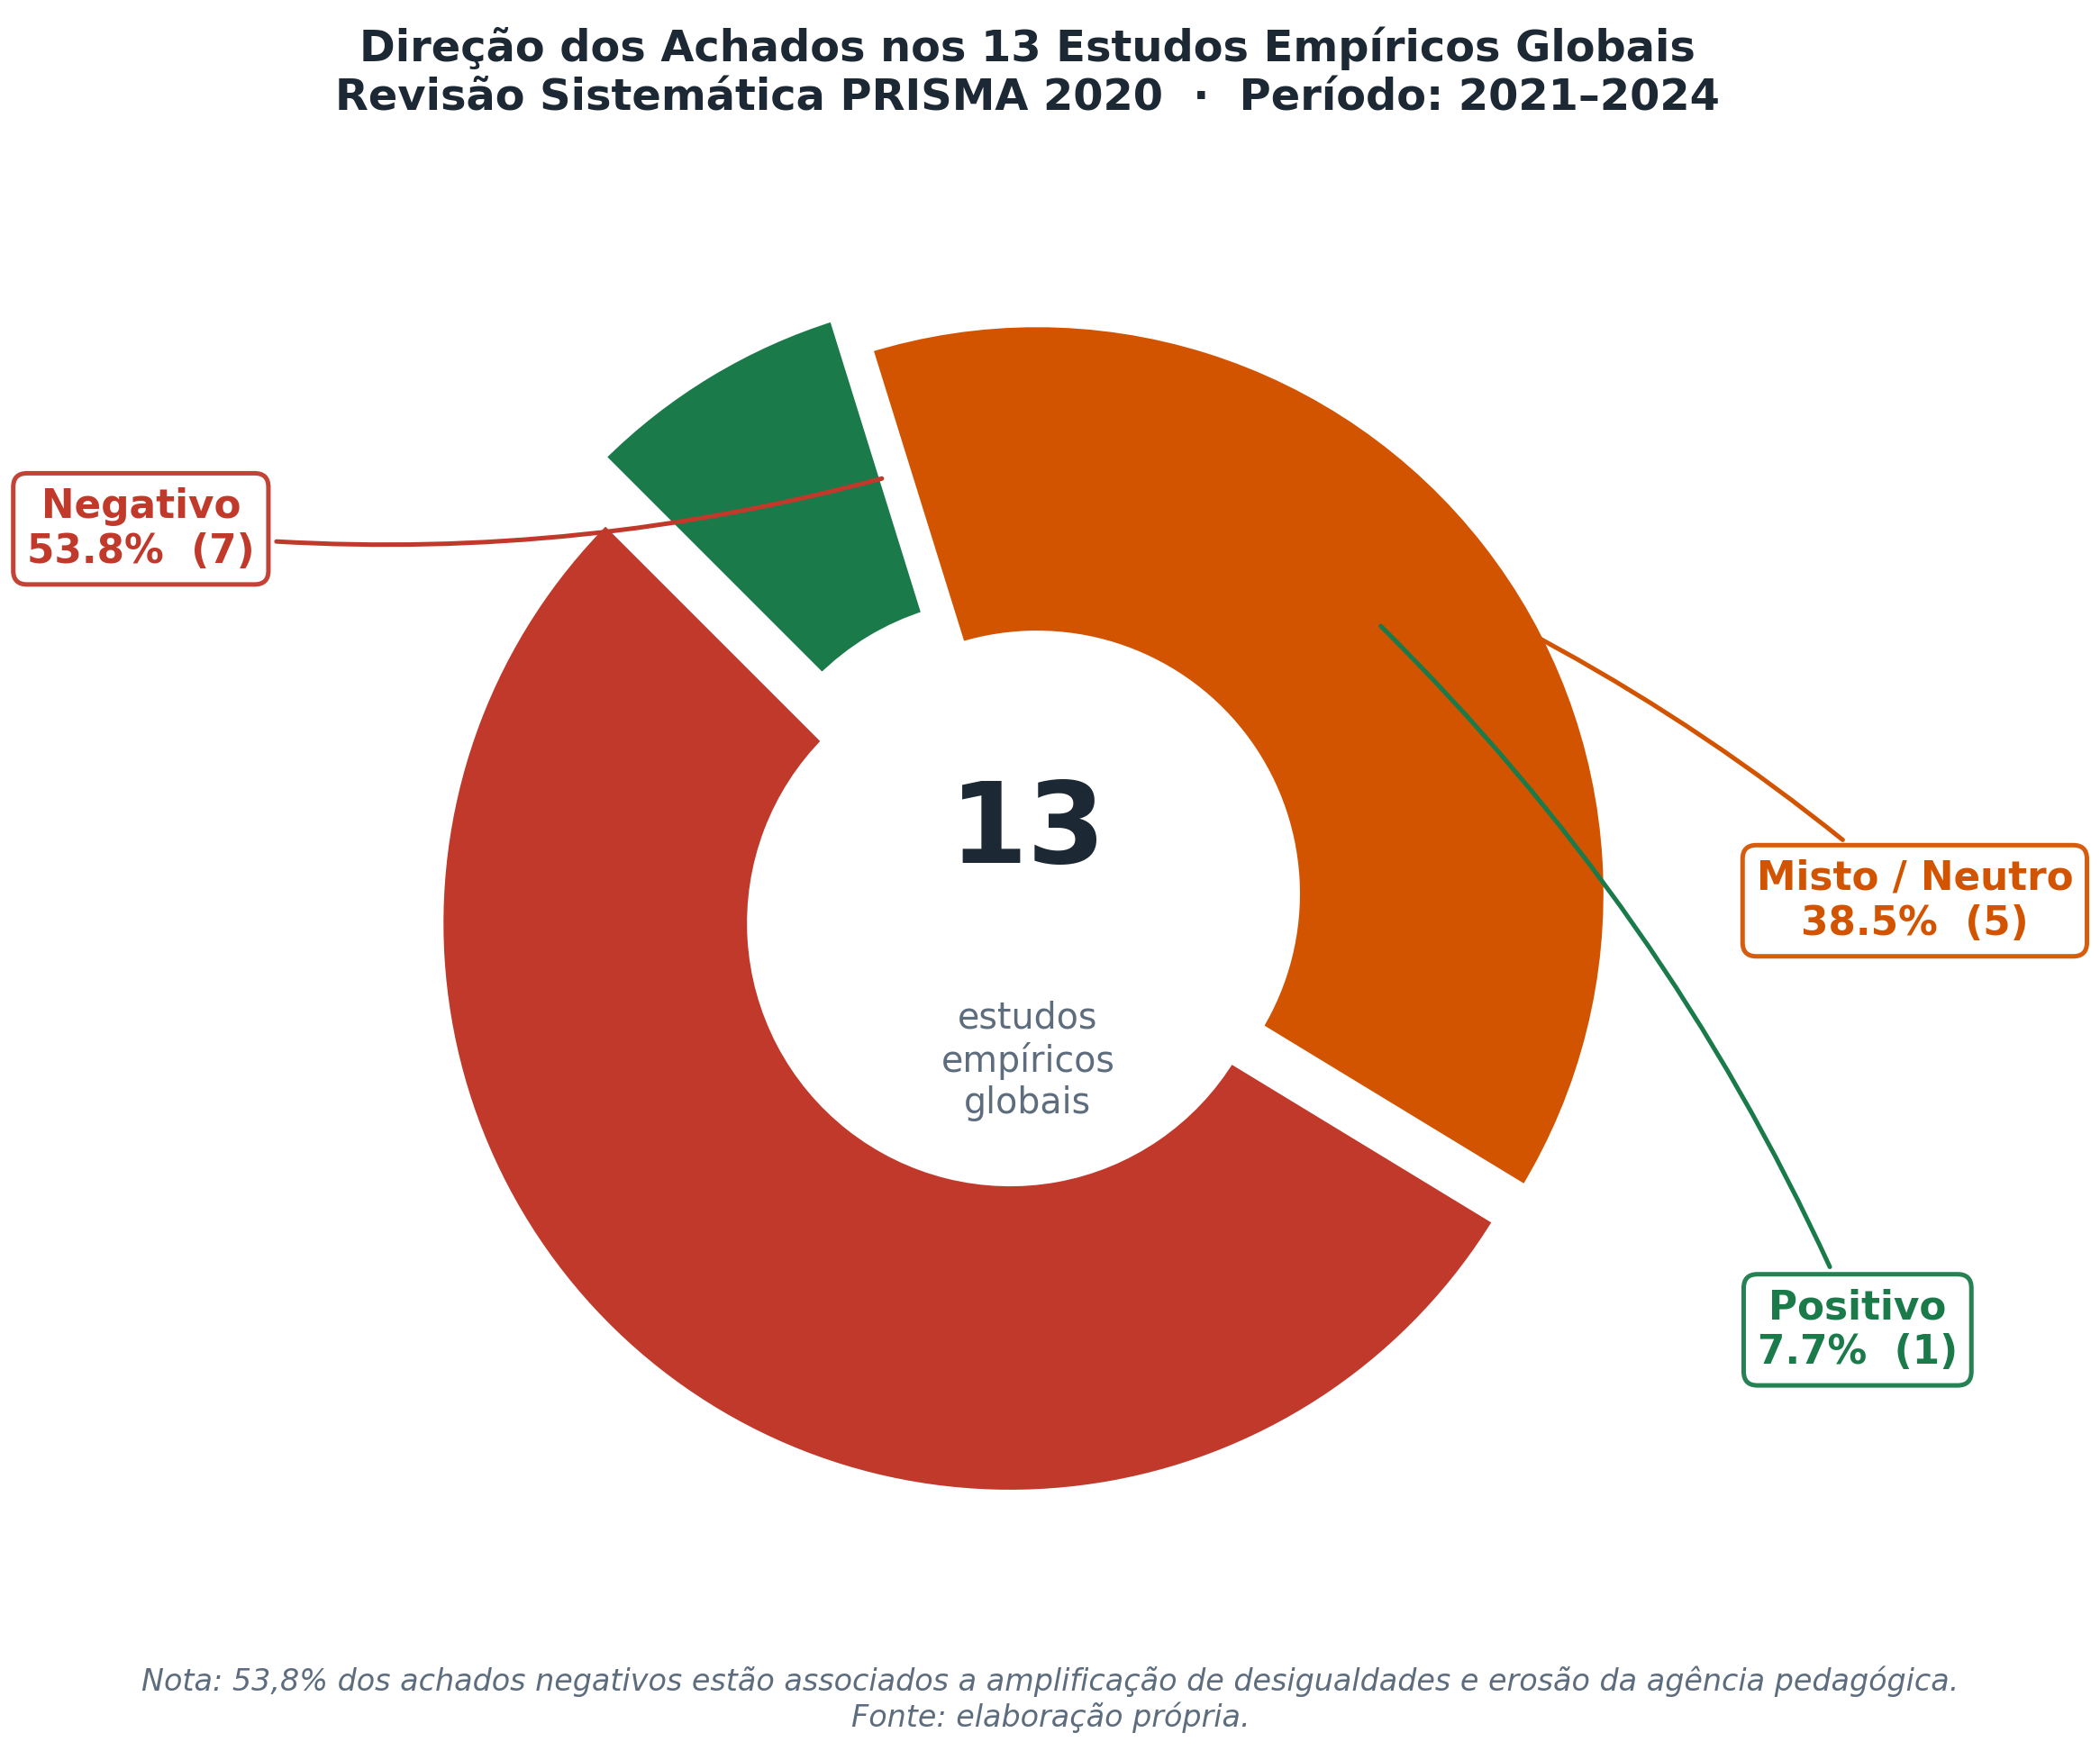
\includegraphics[width=0.68\textwidth]{fig1_empirical_findings.png}
  \caption{Distribuição assimétrica dos achados nos 13 estudos
           empíricos, evidenciando 53,8\% de resultados negativos.}
  \label{fig:donut}
\end{figure}

O corpus final, após a aplicação integral dos critérios de
elegibilidade, compreende 73 artigos, dos quais 13 apresentam
orientação empírica estrita e foram submetidos a análise sistemática
de direção dos achados. A distribuição temática resultante do
processo LDA evidenciou três grandes eixos discursivos no corpus
global — solucionismo tecnológico, iniquidade educacional e
governança algorítmica — cuja inter-relação dialética estrutura
a discussão desenvolvida na seção subsequente.

% -----------------------------------------------------------
\section{Discussão: Infraestrutura como Política, Datificação
         como Extração}
% -----------------------------------------------------------

\subsection{A Dissonância Empírica e o Vácuo Pedagógico}

A primeira constatação relevante que se depreende da análise do
corpus global diz respeito à assimetria entre a retórica de impacto
positivo, predominante nas publicações institucionais e nos materiais
de divulgação corporativa da indústria de EdTech, e os resultados
efetivamente documentados pela investigação científica revisada por
pares. Dentre os 13 estudos com desenho empírico rigoroso, 53,8\%
reportam achados negativos, ao passo que apenas uma minoria documenta
melhorias sustentadas em indicadores de equidade ou desempenho.
Esse dado, antes de revelar uma simples limitação técnica dos sistemas
de IA disponíveis, evidencia a operação de um mecanismo estrutural:
a IA pedagógica, quando inserida em ambientes já marcados por
desigualdades de acesso, de capital cultural e de infraestrutura,
tende a amplificar essas assimetrias, e não a atenuá-las.

A segunda regularidade do corpus é, sob a perspectiva da teoria
social, ainda mais reveladora do que a distribuição dos achados
negativos: 69,2\% dos estudos revisados não especificam o nível de
ensino investigado, tratando a educação como uma massa homogênea e
indiferenciada. Esse vácuo pedagógico não constitui um acidente
metodológico, tampouco uma omissão reparável por ajuste de protocolo;
depreende-se dele a vigência de uma perspectiva tecno-determinista
que, ao abstrair as especificidades do desenvolvimento cognitivo,
das relações pedagógicas situadas e das condições institucionais em
cada etapa formativa, opera com uma concepção de educação funcional
às lógicas da padronização e da escalabilidade algorítmica.
Trata-se, precisamente, do solucionismo que \citet{Morozov2013}
identificou como traço constitutivo do imaginário tecnológico
hegemônico: a solução é concebida antes do problema, e o problema
é reconfigurado retroativamente para adequar-se à solução disponível.

\subsection{Datificação, Colonialismo de Dados e o Caso Brasileiro}

A integração dos dados oriundos do mapeamento nacional evidencia
que a questão da escola pública e da desigualdade estrutural,
presente em 63,3\% do corpus brasileiro, não constitui um tema
periférico ou regional, mas a síntese e o cerne argumentativo
do presente artigo. A predominância dessa temática no debate
acadêmico brasileiro sobre IA educacional expressa um diagnóstico
coletivo que as Ciências Sociais Computacionais permitem mensurar
com precisão: a introdução de sistemas algorítmicos no ensino
público não ocorre num vácuo institucional neutro, mas sobre uma
base de desigualdades estruturais acumuladas historicamente, cuja
lógica de reprodução a IA tende a intensificar, posto que os
sistemas de personalização e de recomendação pedagógica são
invariavelmente treinados sobre dados originários de populações
e contextos radicalmente distintos dos que predominam nas periferias
das cidades brasileiras.

\begin{figure}[htbp]
  \centering
  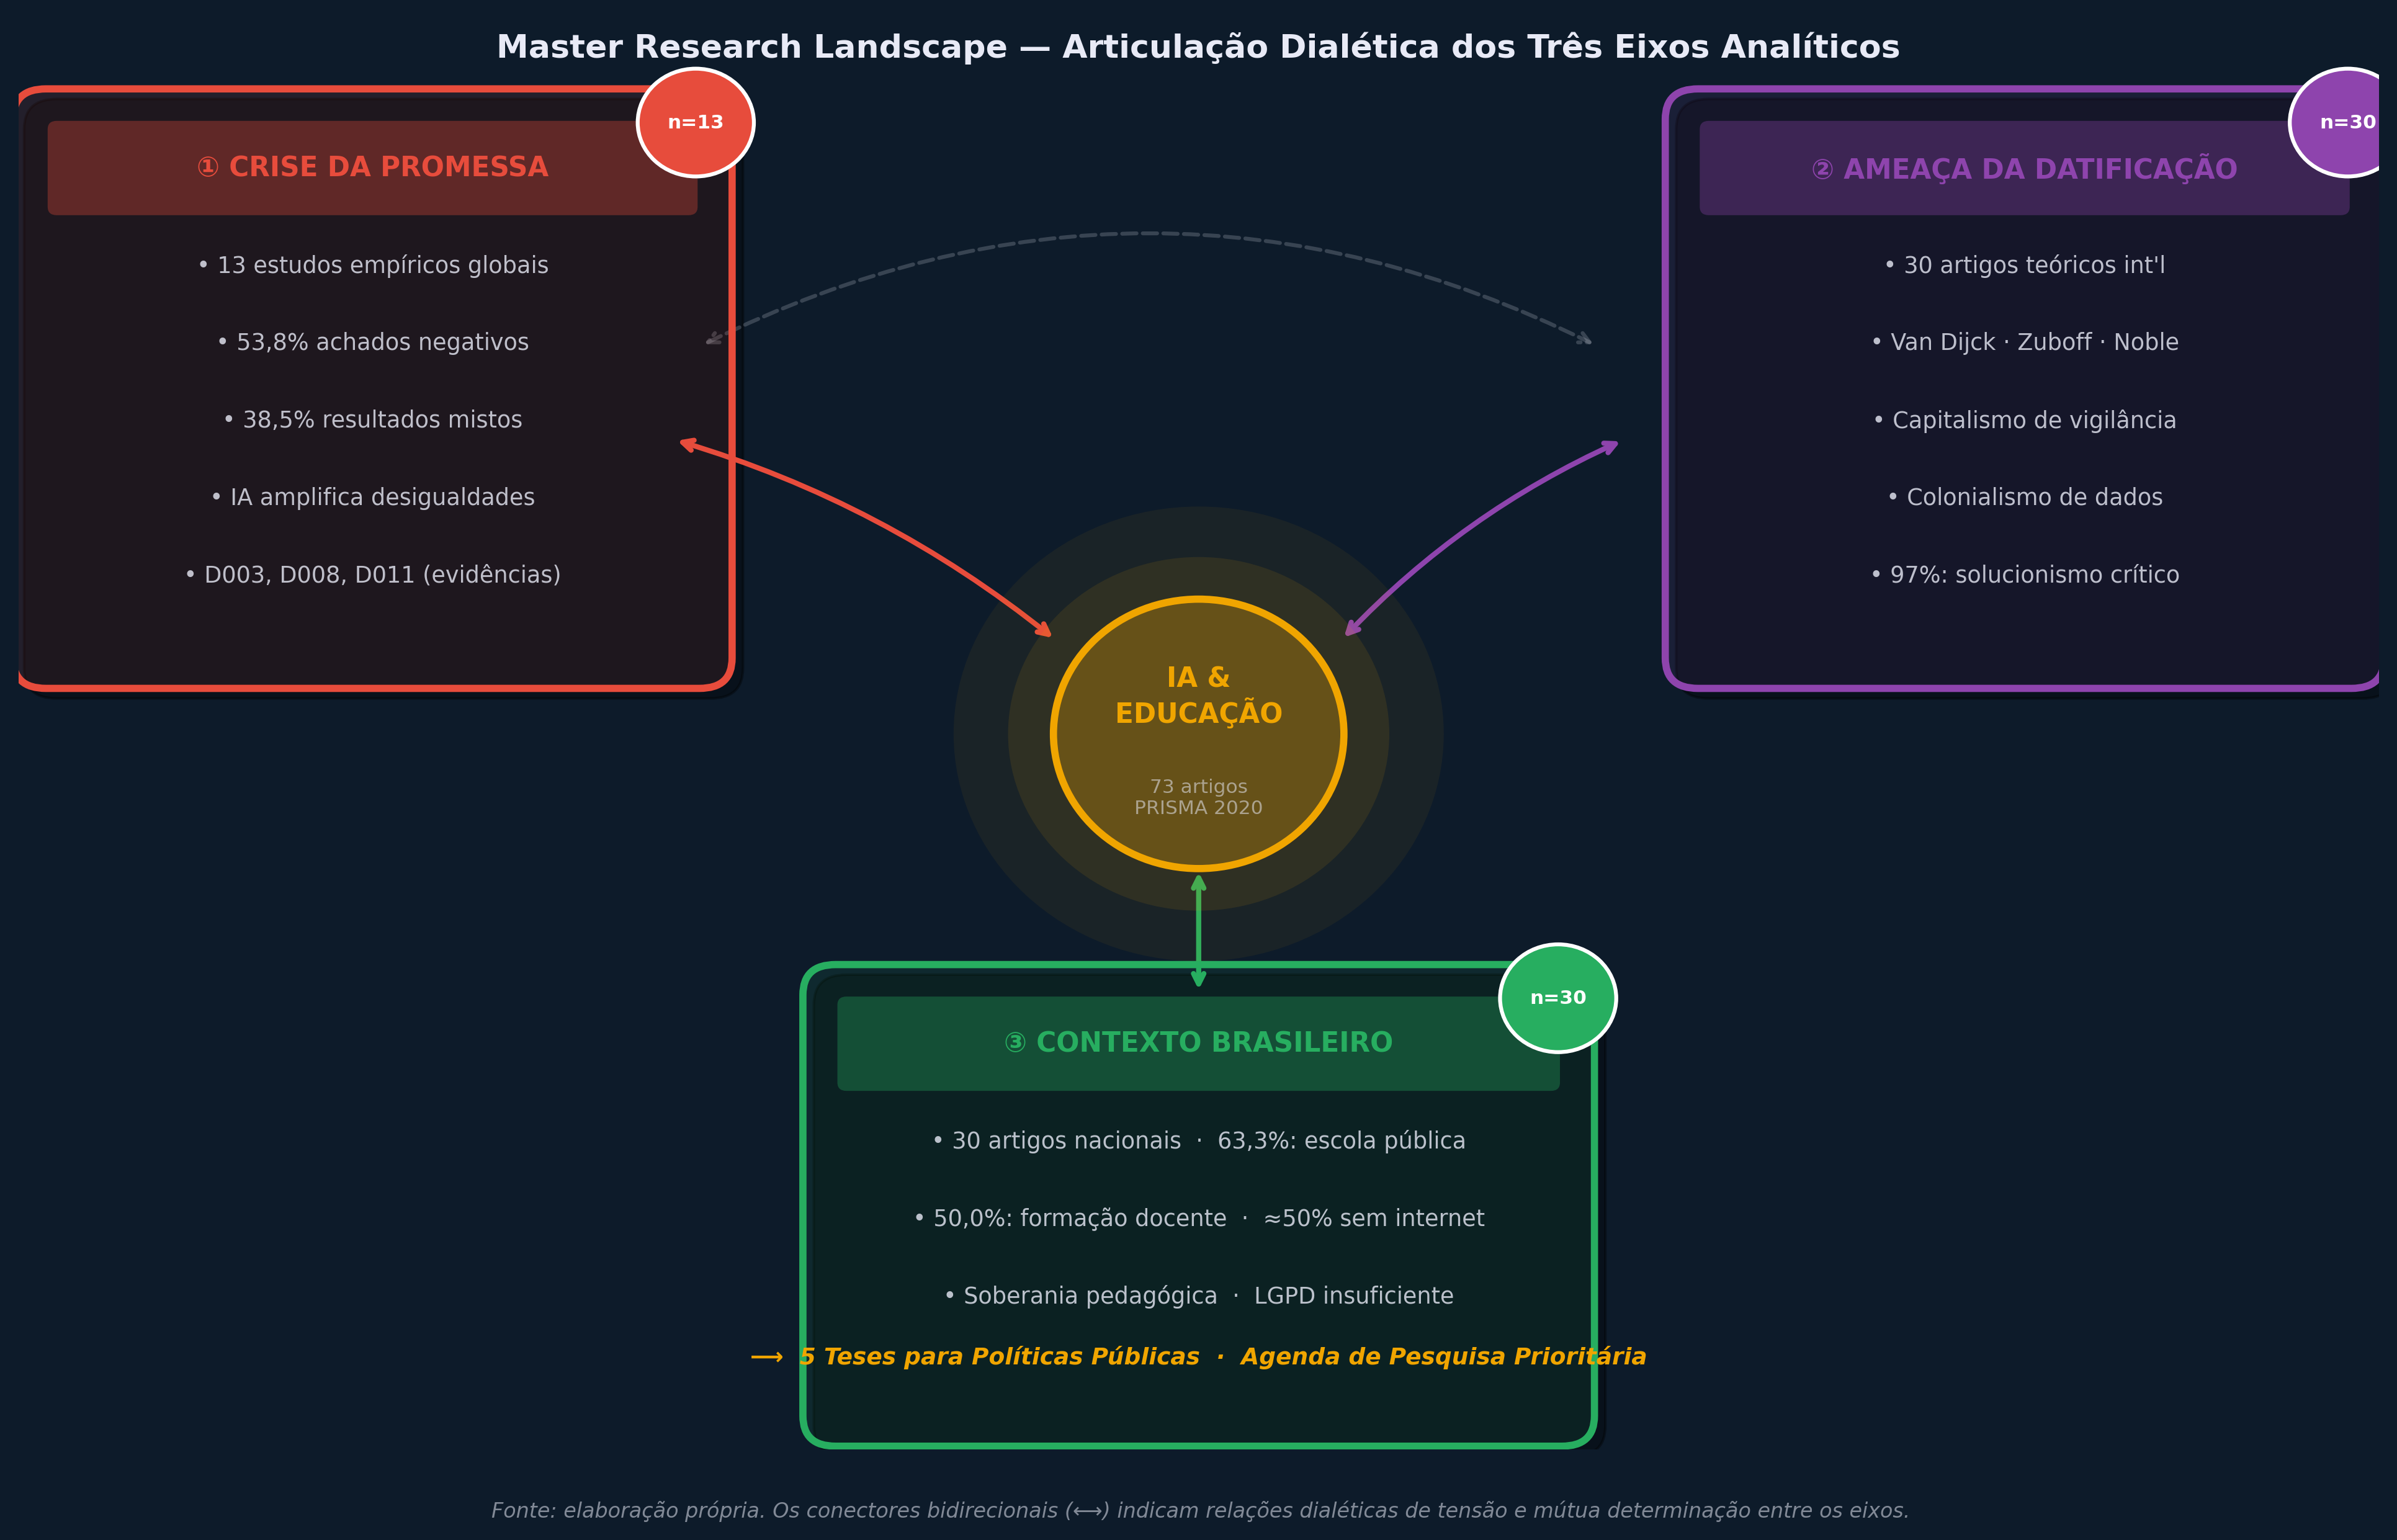
\includegraphics[width=0.95\textwidth]{fig3_dialectical_axes.png}
  \caption{Master Research Landscape: Mapa Conceitual da Pesquisa.
           Integração Dialética entre Evidências Globais,
           Teoria Crítica e Realidade Brasileira.}
  \label{fig:axes}
\end{figure}

A categoria analítica que melhor nomeia essa dinâmica é a de
\textbf{datificação}, entendida, na esteira de \citet{VanDijck2014}
e \citet{Zuboff2019}, como o processo pelo qual fenômenos sociais
— inclusive a aprendizagem, o comportamento discente e as trajetórias
educacionais — são convertidos em dados quantificáveis, armazenados
em infraestruturas privadas e reprocessados como insumo para a
produção de valor econômico e poder preditivo. A escola pública
brasileira, ao adotar plataformas de EdTech desenvolvidas e
hospedadas no Norte Global, insere-se involuntariamente nesse
circuito de extração: as interações cotidianas de 47 milhões de
estudantes convertem-se em matéria-prima para o aprimoramento
de modelos de linguagem e de sistemas de recomendação cujos
benefícios econômicos se concentram em corporações norte-americanas
e europeias, enquanto os custos — em termos de privacidade, de
autonomia pedagógica e de dependência tecnológica estrutural —
recaem sobre as comunidades escolares periféricas.

Essa dinâmica articula o que \citet{CouldryCM2019} denominaram
\textbf{colonialismo de dados}: uma relação assimétrica de poder
na qual territórios e populações do Sul Global figuram, primordialmente,
como provedores de dados brutos para infraestruturas cognitivas
desenvolvidas e controladas pelo Norte. No contexto educacional
brasileiro, o colonialismo de dados assume uma dimensão particularmente
aguda, posto que, quando o currículo, o ritmo de aprendizagem e os
critérios de avaliação são delegados a sistemas algorítmicos opacos,
cujas lógicas de classificação e predição foram treinadas sobre dados
de outras realidades socioculturais, consolida-se uma heteronomia
pedagógica de natureza estrutural. Quem controla o código exerce
poder direto sobre a pedagogia \citep{Noble2018}, e esse controle,
no caso brasileiro, encontra-se sistematicamente fora das instituições
públicas nacionais, das secretarias de educação e das comunidades
docentes.

A ausência de uma infraestrutura digital pública e soberana é, por
conseguinte, um problema político de primeira ordem, que não se
resolve pela simples ampliação do acesso às plataformas disponíveis.
A experiência acumulada nos estados e municípios brasileiros que
adotaram plataformas EdTech privadas sem cláusulas de soberania de
dados demonstra que a captura corporativa não se dá apenas no plano
econômico: ela redefine silenciosamente os objetivos educacionais,
substitui o julgamento docente pelo escrutínio algorítmico e
transforma a relação pedagógica numa cadeia de geração de dados.
A infraestrutura, como sustentou \citet{Winner1980} em sua análise
seminal sobre a política dos artefatos técnicos, não é neutra; ela
incorpora escolhas sobre quem governa, quem é governado e em
benefício de quem o sistema opera. Aplicada ao contexto educacional
brasileiro, essa premissa adquire valência empírica precisa: a
escolha da plataforma é, simultaneamente, uma escolha sobre a
soberania pedagógica.

% -----------------------------------------------------------
\section{Conclusão: A Educação como Resistência à Datificação}
% -----------------------------------------------------------

Os resultados consolidados pela presente revisão sistemática
permitem afirmar, com fundamento empírico e suporte teórico, que a
IA, em seu formato hegemônico atual, opera primordialmente como
vetor de assimetria. A dissonância entre o discurso de transformação
pedagógica e os 53,8\% de achados negativos documentados pela
literatura empírica não resulta de uma fase transitória de adaptação
tecnológica, mas expressa uma contradição estrutural: sistemas
concebidos para maximizar a eficiência e a escalabilidade numa
lógica de mercado tendem, quando inseridos em contextos de
desigualdade pré-existente, a aprofundar as assimetrias que afirmam
combater.

O vácuo pedagógico identificado em 69,2\% dos estudos intensifica
essa contradição, visto que naturaliza a abstração do sujeito
educacional e dissolve as especificidades da relação pedagógica numa
categoria funcional à lógica de padronização algorítmica.
Por conseguinte, a crítica ao solucionismo tecnológico não pode
restringir-se à denúncia do marketing corporativo; ela deve
interrogar os pressupostos epistemológicos que tornam possível
tratar a educação como um problema técnico solucionável por
otimização computacional, desconsiderando as dimensões históricas,
relacionais e políticas que constituem o ato educativo.

No horizonte do Sul Global, e do Brasil em particular, essa
interrogação adquire dimensão política irredutível. A educação
pública, com seus 47 milhões de estudantes, não pode ser concebida
como um mercado a ser capturado pela indústria de EdTech nem como
uma fonte de dados brutos para o aprimoramento de modelos de
linguagem estrangeiros. A resistência à datificação, nesse quadro,
não designa uma posição tecnofóbica nem uma recusa ao desenvolvimento
científico: designa a recusa da heteronomia pedagógica e a afirmação
da agência das comunidades escolares sobre os processos e os produtos
do ato educativo. A construção de infraestruturas digitais públicas,
auditáveis e orientadas pela soberania de dados constitui, destarte,
não uma política setorial de modernização, mas a condição estrutural
sem a qual a inteligência artificial reproduzirá, nos próximos ciclos
tecnológicos, o mesmo padrão de expropriação que a revisão sistemática
aqui apresentada permite, agora, documentar empiricamente.

% -----------------------------------------------------------
\section*{Declaração de Conflito de Interesses}
Os autores declaram ausência de conflito de interesses.

\section*{Financiamento}
A preencher conforme agência financiadora.

\section*{Disponibilidade de Dados e Código}
Repositório: \url{https://github.com/leonardorsl/ia_educacao_research}

% -----------------------------------------------------------
\bibliographystyle{elsarticle-harv}
\bibliography{../references/BIBLIOGRAFIA_MESTRE_IA_EDU}

\end{document}
